\section{Ứng dụng: Phân loại Ảnh (Image Classification)}
\label{sec:image_classification_application}

Sau khi đã mổ xẻ các khối xây dựng cơ bản và các kiến trúc CNN kinh điển cũng như hiện đại, đã đến lúc chúng ta kết hợp chúng lại để giải quyết một trong những bài toán nền tảng, kinh điển và có sức ảnh hưởng nhất trong Thị giác Máy tính: \textbf{Phân loại Ảnh (Image Classification)}.

\subsection{Giới thiệu: Bài toán và Tầm quan trọng}
\label{subsec:classification_intro}
\textbf{Định nghĩa:} Phân loại ảnh là bài toán gán một nhãn (label) duy nhất, từ một tập hợp các lớp (classes) đã được định nghĩa trước, cho toàn bộ một bức ảnh. Nói cách khác, nhiệm vụ của mô hình là nhìn vào một bức ảnh và trả lời câu hỏi: "Đây là gì?".

Mặc dù nghe có vẻ đơn giản, đây là một bài toán cốt lõi vì nhiều lý do:
\begin{itemize}
    \item \textbf{Là "cửa ngõ" cho các bài toán phức tạp hơn:} Nhiều bài toán thị giác phức tạp như phát hiện vật thể (object detection) hay phân đoạn ảnh (image segmentation) thường bắt đầu bằng một "xương sống" (backbone) được huấn luyện trước cho nhiệm vụ phân loại ảnh. Các đặc trưng (features) học được từ bài toán này có tính tổng quát cao và là một điểm khởi đầu tuyệt vời.
    \item \textbf{Là thước đo (benchmark) tiêu chuẩn:} Hiệu năng trên các bộ dữ liệu phân loại ảnh quy mô lớn, đặc biệt là ImageNet, đã và đang là thước đo "vàng" để đánh giá sức mạnh và sự tiến bộ của các kiến trúc mới, từ CNN đến Transformer.
\end{itemize}

\textbf{Các ví dụ ứng dụng phổ biến} của phân loại ảnh trải dài trên mọi lĩnh vực:
\begin{itemize}
    \item \textbf{Trong đời sống hàng ngày:} Các ứng dụng nhận dạng thực vật, động vật; tự động gắn thẻ (tagging) ảnh trong thư viện ảnh cá nhân.
    \item \textbf{Trong y tế:} Phân loại các khối u là lành tính hay ác tính từ ảnh X-quang, MRI; chẩn đoán bệnh về da từ ảnh chụp.
    \item \textbf{Trong thương mại điện tử:} Tự động phân loại sản phẩm vào các danh mục tương ứng từ ảnh người bán tải lên.
    \item \textbf{Trong công nghiệp và nông nghiệp:} Giám sát chất lượng sản phẩm trên dây chuyền, phân loại cây trồng hoặc phát hiện bệnh trên lá cây từ ảnh chụp bằng drone.
\end{itemize}

\subsection{Quy trình Tổng quát của một Hệ thống Phân loại Ảnh}
\label{subsec:classification_pipeline}
Việc xây dựng một hệ thống phân loại ảnh hiệu quả tuân theo một quy trình gồm các bước chuẩn mực trong học máy.

\begin{center}
    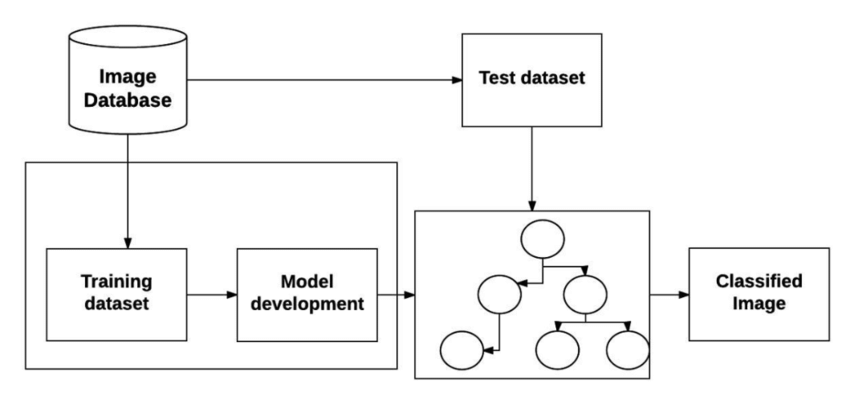
\includegraphics[width=1.0\textwidth]{images/image_classification_pipeline_diagram.png}
    \captionof{figure}{Sơ đồ quy trình tổng quát để xây dựng một hệ thống phân loại ảnh, từ thu thập dữ liệu đến huấn luyện và đánh giá mô hình.}
    \label{fig:image_classification_pipeline}
\end{center}
% Keyword gợi ý: image classification pipeline, deep learning workflow for classification

\begin{enumerate}
    \item \textbf{Thu thập và Chuẩn bị Dữ liệu:}
    Đây là bước quan trọng nhất. "Rác vào, rác ra" (Garbage in, garbage out).
    \begin{itemize}
        \item \textbf{Tập dữ liệu (Datasets):} Sử dụng các bộ dữ liệu công khai như MNIST (chữ số), CIFAR-10/100 (vật thể), ImageNet (1000 lớp vật thể phổ biến), Food-101 (món ăn),... hoặc thu thập dữ liệu riêng cho bài toán cụ thể.
        \item \textbf{Làm sạch và Cân bằng:} Đảm bảo nhãn dữ liệu chính xác và cố gắng cân bằng số lượng mẫu giữa các lớp. Các lớp có quá ít mẫu (lớp thiểu số) có thể khiến mô hình bị thiên vị (biased).
    \end{itemize}

    \item \textbf{Tiền xử lý và Tăng cường Dữ liệu:}
    Đưa dữ liệu về một định dạng chuẩn và làm phong phú nó.
    \begin{itemize}
        \item \textbf{Chuẩn hóa Kích thước:} Thay đổi kích thước (resize) tất cả các ảnh về một kích thước cố định (ví dụ: $224 \times 224$ pixels) mà mô hình yêu cầu.
        \item \textbf{Chuẩn hóa Pixel:} Đưa giá trị của các pixel (thường từ [0, 255]) về một khoảng nhỏ hơn, ví dụ [0, 1] hoặc [-1, 1]. Phổ biến nhất là chuẩn hóa theo trung bình và độ lệch chuẩn của bộ dữ liệu ImageNet, giúp quá trình huấn luyện hội tụ tốt hơn.
        \item \textbf{Tăng cường Dữ liệu (Data Augmentation):} Áp dụng các kỹ thuật đã thảo luận ở Section 3.4 để tạo ra các biến thể của ảnh huấn luyện, giúp mô hình tổng quát hóa tốt hơn.
    \end{itemize}

    \item \textbf{Xây dựng và Lựa chọn Mô hình:}
    Chọn kiến trúc phù hợp cho bài toán.
    \begin{itemize}
        \item \textbf{Chọn Kiến trúc:} Lựa chọn một kiến trúc CNN (như ResNet-50, EfficientNet-B0) hoặc Transformer (như ViT) phù hợp với yêu cầu về độ chính xác và tốc độ.
        \item \textbf{Học chuyển giao (Transfer Learning):} Một chiến lược cực kỳ hiệu quả là không huấn luyện mô hình từ đầu (from scratch). Thay vào đó, ta sử dụng một mô hình đã được huấn luyện trước (pre-trained) trên một bộ dữ liệu rất lớn như ImageNet. Sau đó, ta chỉ cần thay thế lớp phân loại cuối cùng và "tinh chỉnh" (fine-tune) lại một phần hoặc toàn bộ trọng số của mạng trên bộ dữ liệu của mình.
    \end{itemize}

    \item \textbf{Huấn luyện Mô hình:}
    Đây là quá trình tối ưu hóa các trọng số của mô hình.
    \begin{itemize}
        \item \textbf{Hàm mất mát (Loss Function):} Đối với bài toán phân loại đa lớp, hàm mất mát \textbf{Cross-Entropy} là lựa chọn tiêu chuẩn.
        \item \textbf{Thuật toán Tối ưu (Optimizer):} Các thuật toán như Adam, AdamW, hoặc SGD với momentum được sử dụng để cập nhật trọng số của mạng dựa trên gradient của hàm mất mát.
        \item \textbf{Vòng lặp Huấn luyện:} Huấn luyện mô hình qua nhiều \textit{epoch} (mỗi epoch là một lượt duyệt qua toàn bộ tập huấn luyện). Trong mỗi epoch, theo dõi giá trị loss và độ chính xác (accuracy) trên cả tập huấn luyện và tập validation để phát hiện overfitting.
    \end{itemize}

    \item \textbf{Đánh giá và Triển khai:}
    Đo lường hiệu năng và đưa mô hình vào sử dụng.
    \begin{itemize}
        \item \textbf{Thước đo (Metrics):} Sử dụng các thước đo như \textbf{Accuracy}, Precision, Recall, F1-score. Trực quan hóa \textbf{Ma trận Nhầm lẫn (Confusion Matrix)} để hiểu rõ mô hình đang nhầm lẫn giữa các lớp nào.
        \item \textbf{Triển khai (Deployment):} Sau khi hài lòng với hiệu năng, mô hình có thể được tối ưu hóa (ví dụ: lượng tử hóa - quantization) và triển khai trên máy chủ, dịch vụ đám mây, hoặc các thiết bị biên (edge devices).
    \end{itemize}
\end{enumerate}

\subsection{Ví dụ Thực hành với PyTorch}
\label{subsec:pytorch_example}
Dưới đây là một đoạn mã nguồn Python sử dụng thư viện PyTorch để minh họa một quy trình huấn luyện đơn giản cho bài toán phân loại ảnh trên bộ dữ liệu CIFAR-10, sử dụng kỹ thuật học chuyển giao với mô hình ResNet-18.

\begin{minted}[fontsize=\footnotesize, frame=single, linenos=true]{python}
import torch
import torch.nn as nn
import torch.optim as optim
import torchvision.transforms as transforms
import torchvision.datasets as datasets
from torchvision import models

# 1. Tải và Tiền xử lý Dữ liệu
# Định nghĩa các phép biến đổi: thay đổi kích thước, lật ngẫu nhiên,
# chuyển thành tensor và chuẩn hóa theo giá trị của ImageNet.
data_transforms = transforms.Compose([
    transforms.Resize(224),
    transforms.RandomHorizontalFlip(),
    transforms.ToTensor(),
    transforms.Normalize(mean=[0.485, 0.456, 0.406], 
                         std=[0.229, 0.224, 0.225])
])

# Tải bộ dữ liệu CIFAR10 (10 lớp)
train_dataset = datasets.CIFAR10(root='./data', train=True, 
                                 download=True, transform=data_transforms)
train_loader = torch.utils.data.DataLoader(train_dataset, batch_size=64, 
                                           shuffle=True, num_workers=4)

# 2. Xây dựng Mô hình
# Tải mô hình ResNet-18 đã được huấn luyện trước trên ImageNet
model = models.resnet18(pretrained=True)

# "Đóng băng" các lớp đã học để không cập nhật trọng số
for param in model.parameters():
    param.requires_grad = False

# Thay thế lớp phân loại cuối cùng (fully connected layer)
num_ftrs = model.fc.in_features
model.fc = nn.Linear(num_ftrs, 10) # 10 là số lớp của CIFAR-10

# Chuyển mô hình sang GPU nếu có
device = torch.device("cuda:0" if torch.cuda.is_available() else "cpu")
model = model.to(device)

# 3. Định nghĩa Hàm mất mát và Thuật toán Tối ưu
criterion = nn.CrossEntropyLoss()
# Chỉ tối ưu hóa các tham số của lớp cuối cùng mà chúng ta vừa thay thế
optimizer = optim.SGD(model.fc.parameters(), lr=0.001, momentum=0.9)

# 4. Vòng lặp Huấn luyện (Minh họa đơn giản)
num_epochs = 5
for epoch in range(num_epochs):
    model.train() # Đặt mô hình ở chế độ huấn luyện
    running_loss = 0.0
    for inputs, labels in train_loader:
        inputs = inputs.to(device)
        labels = labels.to(device)

        # Xóa các gradient cũ
        optimizer.zero_grad()

        # Forward pass
        outputs = model(inputs)
        loss = criterion(outputs, labels)

        # Backward pass và tối ưu hóa
        loss.backward()
        optimizer.step()

        running_loss += loss.item() * inputs.size(0)

    epoch_loss = running_loss / len(train_dataset)
    print(f"Epoch {epoch+1}/{num_epochs}, Loss: {epoch_loss:.4f}")

print("Finished Training")
\end{minted}

\subsection{Các Thách thức và Xu hướng Mới}
\label{subsec:classification_challenges_trends}
Mặc dù phân loại ảnh là một bài toán đã "gần như được giải quyết" trên các bộ dữ liệu benchmark, các thách thức trong thế giới thực vẫn còn rất nhiều.

\begin{itemize}
    \item \textbf{Mất cân bằng Dữ liệu (Data Imbalance):} Trong thực tế, số lượng mẫu giữa các lớp thường chênh lệch rất lớn. Các kỹ thuật như oversampling (tạo thêm mẫu cho lớp thiểu số), undersampling, hoặc sử dụng các hàm mất mát đặc biệt như Focal Loss được dùng để giải quyết.
    \item \textbf{Suy luận Hiệu quả (Efficient Inference):} Yêu cầu chạy mô hình trên các thiết bị có tài nguyên hạn chế (điện thoại, camera thông minh) đã thúc đẩy sự phát triển của các kiến trúc nhẹ như MobileNet, EfficientNet-Lite, và các kỹ thuật như lượng tử hóa, cắt tỉa (pruning).
    \item \textbf{Tính Bền vững và Khả năng Diễn giải (Robustness \& Explainability):} Các mô hình CNN có thể dễ dàng bị "đánh lừa" bởi các nhiễu loạn nhỏ (adversarial attacks). Việc hiểu "tại sao" mô hình đưa ra một dự đoán (sử dụng các kỹ thuật như Grad-CAM, LIME) và làm cho nó bền vững hơn đang là một hướng nghiên cứu tích cực.
    \item \textbf{Phân loại Zero-shot/Few-shot:} Với sự trỗi dậy của các \textbf{mô hình nền tảng (foundation models)} đa phương thức như CLIP, chúng ta có thể phân loại ảnh vào các lớp mới mà không cần huấn luyện lại hoặc chỉ cần một vài ví dụ. Đây là một sự thay đổi mô thức, chuyển từ việc huấn luyện các mô hình chuyên biệt sang việc "prompting" các mô hình tổng quát lớn.
\end{itemize}

\section*{Tài liệu tham khảo}
\begin{itemize}
    \item[1] Krizhevsky, A., Sutskever, I.,\& Hinton, G. E. (2012). ImageNet classification with deep convolutional neural networks. In \textit{Advances in neural information processing systems (NIPS)}. (Paper gốc về AlexNet, khởi đầu cho việc sử dụng CNN sâu cho phân loại ảnh quy mô lớn).
    \item[2] He, K., Zhang, X., Ren, S.,\& Sun, J. (2016). Deep residual learning for image recognition. In \textit{Proceedings of the IEEE conference on computer vision and pattern recognition (CVPR)}. (Paper về ResNet, một trong những kiến trúc xương sống phổ biến nhất cho phân loại ảnh).
    \item[3] Tan, M.,\& Le, Q. V. (2019). Efficientnet: Rethinking model scaling for convolutional neural networks. In \textit{International Conference on Machine Learning (ICML)}. (Paper về EfficientNet, thiết lập state-of-the-art về sự cân bằng giữa độ chính xác và hiệu quả).
    \item[4] Dosovitskiy, A., Beyer, L., Kolesnikov, A., Weissenborn, D., Zhai, X., Unterthiner, T., ...\& Houlsby, N. (2020). An image is worth 16x16 words: Transformers for image recognition at scale. \textit{arXiv preprint arXiv:2010.11929}. (Paper gốc về Vision Transformer - ViT).
    \item[5] Radford, A., Kim, J. W., Hallacy, C., Ramesh, A., Goh, G., Agarwal, S., ...\& Sutskever, I. (2021). Learning transferable visual models from natural language supervision. In \textit{International Conference on Machine Learning (ICML)}. (Paper gốc về CLIP, một mô hình nền tảng cho phân loại zero-shot).
    \item[6] Selvaraju, R. R., Cogswell, M., Das, A., Vedantam, R., Parikh, D.,\& Batra, D. (2017). Grad-cam: Visual explanations from deep networks via gradient-based localization. In \textit{Proceedings of the IEEE international conference on computer vision (ICCV)}. (Giới thiệu Grad-CAM, một kỹ thuật phổ biến để diễn giải các quyết định của CNN).
\end{itemize}